\chapter { Developer Tooling }

Providing great developer tooling can endow even the most anemic processor with outsized capabilities \cite{nytimes_doom_ports_2025}\cite{evans_wasm_microcontrollers}. To promote the authoring and distribution of WASM-based audio DSP modules with a smooth developer experience (DX), I have created a proof-of-concept development environment that runs entirely client-side in the browser.

A contributor to the siloed nature of many embedded systems is their scattered development environments. To provide a glimpse into the status quo of the field circa 2005, I present a quote from \cite{catsoulis2005designing}:

\begin{quotation}
When you're developing your embedded system, it is best to start with a
development kit from the processor's manufacturer [...] it should [...]
include a nice Integrated Development Environment (or IDE). [...]

Some of these companies do a fantastic job, while others seem to employ
stray chimpanzees as design engineers. [...]

Almost without exception, the IDEs will run on only one platform and
under only one operating system. No prizes for guessing which one.
So, if your preferred environment is a Unix workstation, generally
you're out of luck.
\end{quotation}

Fortunately for contemporary programmers, developer tooling for embedded systems has become much more friendly. The advent of Arduino\cite{arduino} demonstrated that the application of design principles from creative coding tools to embedded systems can fuel major innovation by enfranchising more developers.

% PARAGRAPH ABOUT WEB-BASED IDEs (FAUST, Stanford).
Exemplary developer tooling geared towards enfranchisement of new programmers can be found in web-based IDEs, which have gained prominence in the past decade as highly accessible tools for people learning computer programming\cite{6654478}\cite{delgadillo2025fully}. A major advantage of web-based IDEs is that they are consistent across operating systems, increasing ease of setup compared to local development tools. WASM-based audio DSP modules lend themselves well to a web-based IDE, as WASM produced by developers' code can be rapidly auditioned using the Web Audio API. Notable audio-focused web-based IDEs exist for the FAUST\cite{ren2019faust} and ChucK\cite{mulshine2023webchuck} audio DSLs, but not for C/C++, Rust, and other popular languages for audio.

In 2025 I began work on a web-based IDE for writing and auditioning C/C++ audio code in the browser, entitled Hear-C\cite{Hear-Crepo}. My initial architecture relied on a server for compiling C/C++ to WASM using Emscripten, but discovery of \lstinline{wasm-clang}\cite{binji_wasm_clang}, a C/C++ to WASM compiler itself compiled to WASM, enabled me to remove dependency on a server.

% and coding has been made more accessible through creative coding tools, etc.

% Programming MCUs from browser? Arduino Cloud Editor, https://ieeexplore.ieee.org/abstract/document/7732276?casa_token=V4fkp3u1ZKQAAAAA:fa_7C4UVCplEQ4H1QoJekgywY7s4Vn2bCKu4sRRoDY-U0z887ukbTsvvLnGZ9vXf1jIqrcI, etc

Given the promising performance demonstrated by Web Assembly Micro Runtime (WAMR) in Chapter~\ref{sec:bench}, I investigated the possibility of compiling its open-source \lstinline{wamrc} compiler (which translates WASM to WAMR AOT modules) itself to WASM. This proved highly doable within a span of a few days leveraging agentic coding tools.

% I leveraged it to build a platform for developing and auditioning C/C++ audio code in the browser, and flashing the resulting program to the Daisy Seed.

In a fork of Hear-C, I added the functionality to transpile WASM to WAMR AOT via the WASM-compiled \lstinline{wamrc}, as well as tools for flashing and running the resulting modules on the Daisy Seed. Though I focused on the Daisy (WAMR AOT for ARM Cortex M7), the WASM-compiled \lstinline{wamrc} I have published supports the full range of ARM Cortex M and A series processors that a standard build of \lstinline{wamrc} does. I disabled other targets (\lstinline{aarch64}, \lstinline{x86_64}, \lstinline{riscv32}, etc) via build system flags due to time constraints, but expect that these would be relatively easy to add in the future. Source code for the web-based IDE can be found at \cite{DaisyOnlinerepo}.

\begin{figure}[ht]
\vspace{12pt}
\centerline{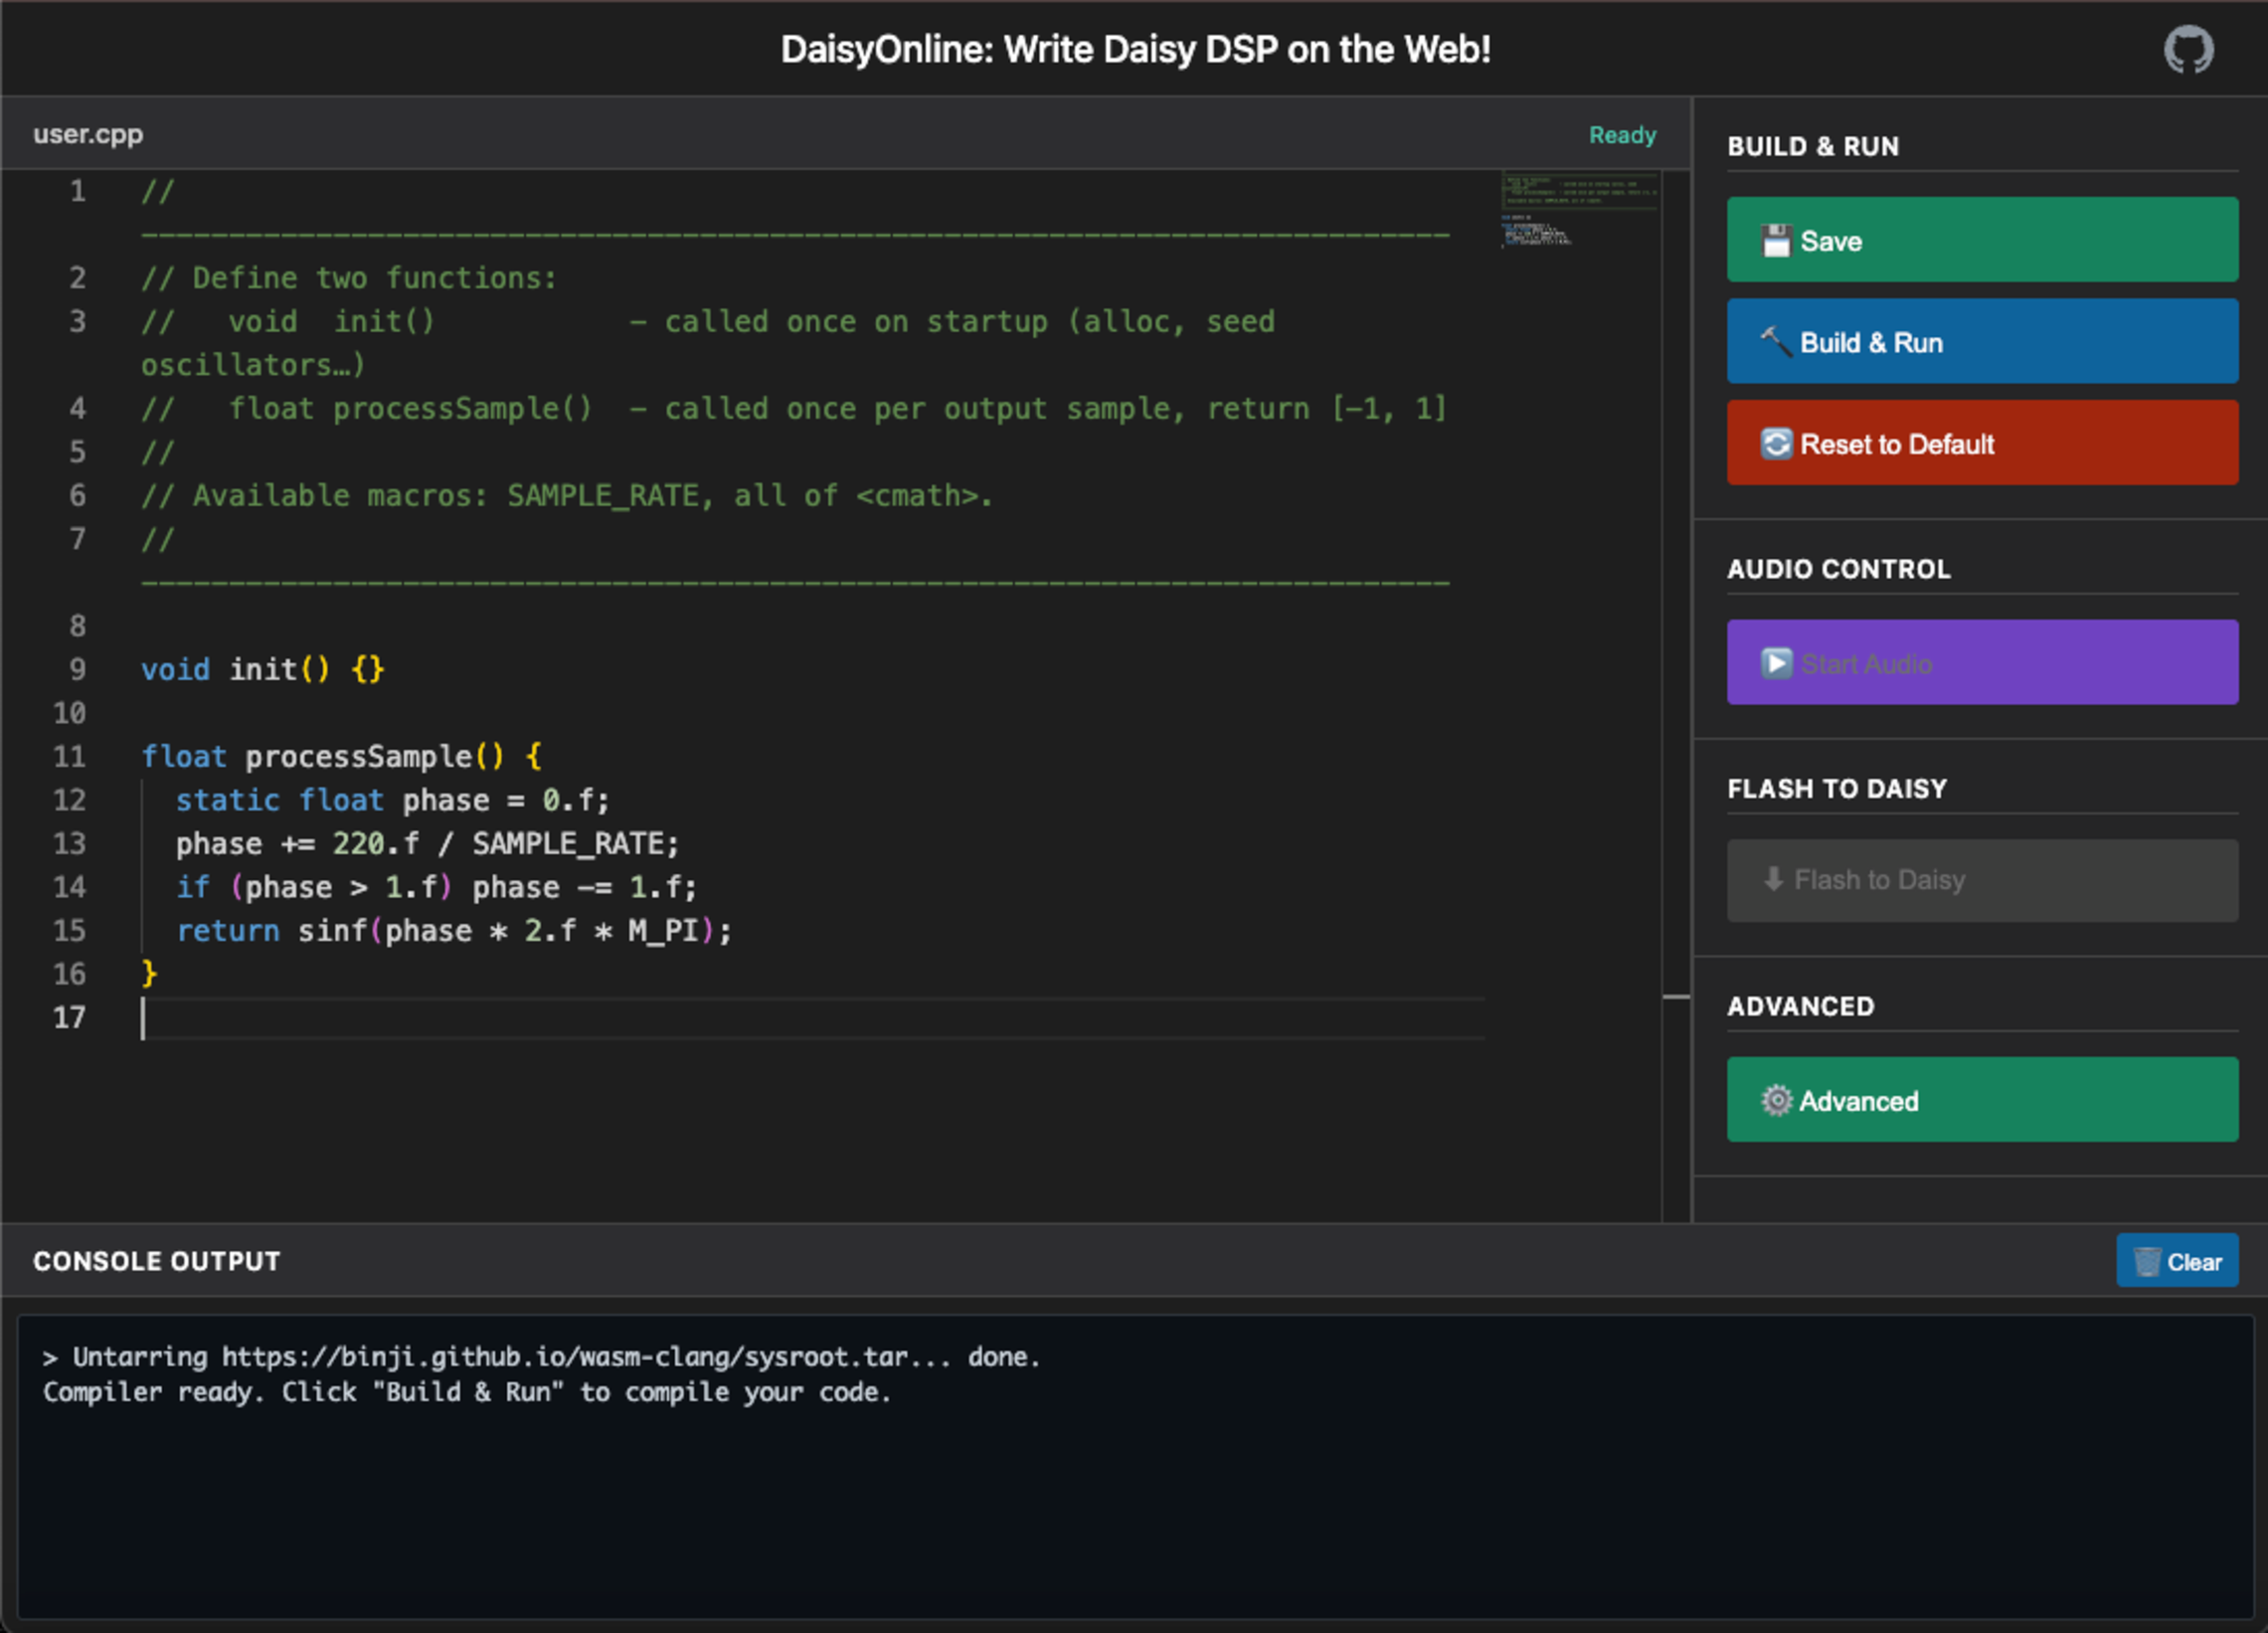
\includegraphics[scale=0.4]{figures/DaisyOnline.pdf}}
\caption{\label{DaisyOnline}{\it DaisyOnline, an online IDE for developing and deploying WebAssembly on the Daisy Seed}}
\end{figure}
